\documentclass[10pt,a4paper]{article}
\usepackage[natbibapa]{apacite} 
\usepackage{amsmath}
\usepackage{tikz}
\bibliographystyle{apacite}

\title{Assignment 2 Machine Learning COS4852}
\author{ Adriaan Louw (53031377) }

\tikzset{
  treenode/.style = {shape=rectangle, rounded corners,
                     draw, align=center,
                     top color=white, bottom color=blue!20},
  root/.style     = {treenode, font=\Large, bottom color=red!30},
  env/.style      = {treenode, font=\ttfamily\normalsize},
  dummy/.style    = {circle,draw}
}

\usetikzlibrary{shapes.misc}

\tikzset{cross/.style={cross out, draw=black, minimum size=20*(#1-\pgflinewidth), inner sep=0pt, outer sep=0pt},
%default radius will be 1pt. 
cross/.default={1pt}}


\tikzset{basic/.style={draw,fill=blue!50!green!20,
                       text badly centered,minimum width=3em}}
\tikzset{input/.style={basic,circle}}
\tikzset{weights/.style={basic,rectangle,minimum width=2em}}
\tikzset{functions/.style={basic,circle,fill=blue!50!green!20}}
\newcommand{\addsymbol}{\draw[thick] (0.5em,0.5em) -- (0,0.5em) -- 
                        (0,-0.5em) --  (-0.5em,-0.5em)
                        (0em,0.75em) -- (0em,-0.75em)
                        (0.75em,0em) -- (-0.75em,0em);}
\begin{document}

\maketitle

\tableofcontents

\section{Question 1}
\subsection{Question 1(a)}

Firstly we calculate the line 

\begin{equation}
\label{line}
 x_2 = mx_1 + c
\end{equation}

for the intersect points (2,0) and (0,6).

Calculating slope m,

\begin{equation}
\begin{split}
m &= \frac{6-0}{0-2} \\
  &= -3\\
\end{split}
\end{equation}

$x_2$ intercept $c$ is 6.

This makes equation \ref{line}

\begin{equation}
\label{pop}
x_2 = -3x_1 + 6
\end{equation}

\cite{nils} gives the equation for the hyperplane as

\begin{equation}
\sum_{i=1}^n x_i\omega_i \geq \theta
\end{equation}

which in this case gives the equation for the hyperplane to be

\begin{equation}
\label{weightline}
\omega_1x_1 + \omega_2x_2 +\omega_3 = 0
\end{equation}

We need to get equation \ref{weightline} in the form of equation \ref{line}

\begin{equation}
\begin{split}
\label{simp}
\omega_1x_1 + \omega_2x_2 + +\omega_3 &= 0\\
\omega_2x_2 &= -\omega_1x_1 - \omega_3\\ 
x_2 &= -\frac{\omega_1x_1}{\omega_2} - \frac{\omega_3}{\omega_2} \\ 
\end{split}
\end{equation}

Comparing coefficients m and c from equation \ref{pop} to \ref{simp} we get

\begin{equation}
\begin{split}
-\frac{\omega_1}{\omega_2} &= -3 \\
\omega_1 &= 3\omega_2\\ 
\end{split}
\end{equation}

and

\begin{equation}
\begin{split}
-\frac{\omega_3}{\omega_2} &= 6\\
\omega_3 &= -6\omega_2\\ 
\end{split}
\end{equation}

If we choose $\omega_3 = -2$ then $\omega_1=1$ and $\omega_2 = \frac{1}{3}$. This makes the hyperplane equation from equation \ref{weightline}

\begin{equation}
x_1 + \frac{x_2}{3} -2 = 0
\end{equation}

Now we need to test this hyperplane. For positive instance (2,6)

\begin{equation}
\begin{split}
x_1 + \frac{x_2}{3} - 2 &= \\
2 + \frac{6}{2} - 2 &= \\
2&\\
\end{split}
\end{equation}

Which is as expected.

And the negative instance (-1,2)

\begin{equation}
\begin{split}
x_1 + \frac{x_2}{3} - 2 &= \\
-1 + \frac{2}{3} -2 & = \\
-\frac{7}{3}
\end{split}
\end{equation}

This is also as expected. The perceptron now classifies the the data correctly
\subsection{Question 1(b)}

\begin{center}
\begin{tikzpicture}[scale=0.6]
%\draw [help lines] (-3,-3) grid (3,3);
% Euclidean
\draw [<->](0,-8)--(0,8) node[right]{$X_2$};
\draw [<->](-8,0)--(8,0) node[right]{$X_1$};
 
%labels
\foreach \x in {-8,-6,-4,-2,2,4,6,8}
     \draw (\x,1pt) -- (\x,-3pt) node[anchor=north] {$\x$};

\foreach \y/\ytext in {-8,-6,-4,-2,2,4,6,8}
     \draw (1pt,\y) -- (-3pt,\y) node[anchor=east] {$\y$};
 
\draw (-1,2) node[cross,green]{};
\draw (1,-2) node[cross,green]{};
\draw (-2,-5) node[cross,green]{};
\draw (-5,-2) node[cross,green]{}; 

\draw (-5,6) node[cross,red]{};
\draw (3,5) node[cross,red]{};
\draw (2,-2) node[cross,red]{};
\draw (5,-5) node[cross,red]{};

\draw [blue] (-8,8) -- (8,-8);
\draw [teal] (-8,66/7) -- (8,-62/7);
 
\end{tikzpicture}
\end{center}

From the above image we can see that any that it is not possible to create a hyperplane that correctly classifies all negative instances and positive instances. The blue line is the line $x_2 = -x_1$ and the teal line is the line $x_2 = -\frac{7}{8}x_1 + \frac{2}{7}$. The any minimum plane that correctly classifies all the negative instances will classify the positive instance (-1,2) incorrectly as negative. 

We can create a hyperplane from regression from all the points close to where the hyperplane should be. Using negative points (-5,6),(2,-2),(5,-5) and positive points (-1,2),(1,-2)

For the equation of the regressed line $x_2=mx_1+c$

\begin{equation}
\begin{split}
\label{m}
m &= r\frac{S(x_2)}{S(x_1)}\\ 
m &= \frac{\sum((x_1 - \bar{x_1})(x_2-\bar{x_2}))}{\sqrt{\sum (x_1-\bar{x_1})^2 \sum(x_2-\bar{x_2})^2}} \frac{\sqrt{\frac{\sum (x_2-\bar{x_2})^2}{n-1}}}{\sqrt{\frac{\sum (x_1-\bar{x_1})^2}{n-1}}}\\
\end{split}
\end{equation}

where r is Pearsons Correlation Coefficient and S is standard deviation of axis $x_2$ or $x_1$.

Here follows the calculation

\begin{tabular}{|c|c|c|c|c|c|c|}
\hline
$x_1$ & $x_2$ & $x_1-\bar{x_1}$ & $x_2-\bar{x_2}$ &$(x_1-\bar{x_1})(x_2-\bar{x_2})$ & $(x_1-\bar{x_1})^2$ & $(x_2-\bar{x_2})^2$ \\ 
\hline
-5 &  6 & -5.4 &  6.2 & -33.48 & 29.16 & 38.44\\
 2 & -2 &  1.6 & -1.8 &  -2.88 &  2.56 &  3.24\\
 5 & -5 &  4.6 & -4.8 & -22.08 & 21.16 & 23.04\\
-1 &  2 & -1.4 &  2.2 &  -3.08 &  1.96 &  4.84\\
 1 & -2 &  0.6 & -1.8 &  -1.08 &  0.36 &  3.24\\
\hline
\end{tabular}

From the above table we have $\bar{x_1} = 0.4, \bar{x_2} = -0.2, \sum((x_1 - \bar{x_1})(x_2-\bar{x_2})) = -62.6, (x_1-\bar{x_1})^2 = 55.2,and (x_2-\bar{x_2})^2 = 72.8$ 

Passing these into equation \ref{m} we get m = -1.13

\begin{equation}
\begin{split}
c &= \bar{x_2} - m\bar{x_1}\\
  &= -0.2 - (-1.13)(0.4)\\
  &= 0.25\\  
\end{split}
\end{equation}

Which gives us equation 

\begin{equation}
x_2 = -1.13x_1 + 0.25
\end{equation}

Visually it would be

\begin{center}
\begin{tikzpicture}[scale=0.6]
%\draw [help lines] (-3,-3) grid (3,3);
% Euclidean
\draw [<->](0,-8)--(0,8) node[right]{$X_2$};
\draw [<->](-8,0)--(8,0) node[right]{$X_1$};
 
%labels
\foreach \x in {-8,-6,-4,-2,2,4,6,8}
     \draw (\x,1pt) -- (\x,-3pt) node[anchor=north] {$\x$};

\foreach \y/\ytext in {-8,-6,-4,-2,2,4,6,8}
     \draw (1pt,\y) -- (-3pt,\y) node[anchor=east] {$\y$};
 
\draw (-1,2) node[cross,green]{};
\draw (1,-2) node[cross,green]{};
\draw (-2,-5) node[cross,green]{};
\draw (-5,-2) node[cross,green]{}; 

\draw (-5,6) node[cross,red]{};
\draw (3,5) node[cross,red]{};
\draw (2,-2) node[cross,red]{};
\draw (5,-5) node[cross,red]{};

\draw [blue] (-8,9.32) -- (8,-8.81);
 
\end{tikzpicture}
\end{center}

This will minimise the error even though it would incorrectly classify (-1,2)

\subsection{Question 1(c)}
\subsection{Question 1(d)}

\section{Question 2}
\subsection{Question 2(a)}

The truth table for this function is
 
\begin{tabular}{|c|c|c|c|}
\hline
$x_1$ & $x_2$ & $\neg x_1$ & $\neg x_1 \vee x_2$ \\
\hline
-1 &-1 &1 &-1\\
-1 &1 &1 &1\\
1 &-1 &-1 &-1\\
1 &1 &-1 &-1\\
\hline
\end{tabular}

Visually this is:

\begin{center}
\begin{tikzpicture}[scale=3.0]
%\draw [help lines] (-3,-3) grid (3,3);
% Euclidean
\draw [<->](0,-1.1)--(0,1.1) node[right]{$x_2$};
\draw [<->](-1.1,0)--(1.1,0) node[right]{$x_1$};
 
\draw[teal,thick,dashed] (-1.0,-0.5) -- (0.5,1.0);

%labels
\foreach \x in {-1,1}
     \draw (\x,1pt) -- (\x,-3pt) node[anchor=north] {$\x$};

\foreach \y/\ytext in {-1,1}
     \draw (1pt,\y) -- (-3pt,\y) node[anchor=east] {$\y$};
 
\draw (-1,-1) node[cross,red]{};
\draw (-1,1) node[cross,green]{};
\draw (1,-1) node[cross,red]{};
\draw (1,1) node[cross,red]{}; 

\end{tikzpicture}
\end{center}

The dashed line represents the function

\begin{equation}
x_2 = x_1 + 0.5
\end{equation}

This hyperplane will classify the boolean function correctly because it linearly separates all the positive instances from the negative ones.

The equation for the hyperplane with weights are given by equation \ref{weightline} and we know from equation \ref{simp} what the relationship is from the weight equation to the line equation. Thus for case

\begin{equation}
\begin{split}
m &= -\frac{\omega_1}{\omega_2} \\
1 &= -\frac{\omega_1}{\omega_2} \\
\omega_2 &= -\omega_1 \\
\end{split}
\end{equation}

and

\begin{equation}
\begin{split}
c &= -\frac{\omega_0}{\omega_2}\\
0.5 &= -\frac{\omega_0}{\omega_2}\\
\omega_0 &= -\frac{\omega_2}{2}\\
\end{split}
\end{equation}

Now we have the relationship between the weights. If we try $\omega_0 = 1$ we get $\omega_1 = 2$ and $\omega_2 = -2$ 

Which makes our weight equation

\begin{equation}
2x_1 - 2x_2 + 1
\end{equation}

Testing for polarity with point (-1,-1) we get
\begin{equation}
\begin{split}
2(-1) -2(-1) + 1 &= 1
\end{split}
\end{equation}

which indicates a positive result but we expect a negative result. Thus our polarity is wrong

We try $\omega_0 = -1$ which gives $\omega_1 = -2$ and $\omega_2 = 2$

Which makes the weight equation

\begin{equation}
-2x_1 + 2x_2 - 1
\end{equation}

Trying all our data we can sum it up in the following table

\begin{tabular}{|c|c|c|}
\hline
$x_1$ & $x_2$ & Result \\
\hline
-1 &-1 & -1\\
-1 & 1 & 4\\
1  &-1 & -5\\
1  & 1 & -1 \\
\hline
\end{tabular}

This shows that weights $\omega_0 = -1$; $\omega_1 = -2$ and $\omega_2 = 2$ correctly classify the data

 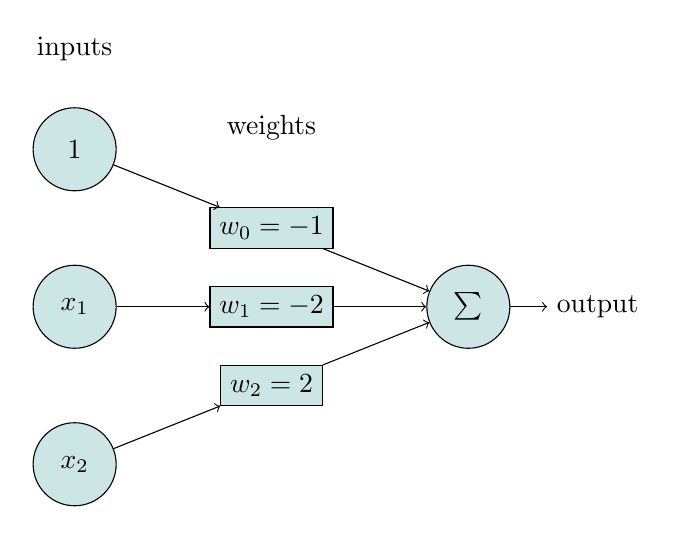
\begin{tikzpicture}[scale=1]
    \foreach \h [count=\hi ] in {$x_2$,$x_1$,$1$}{%
          \node[input] (f\hi) at (0,\hi*2cm-4 cm) {\h};
        }
    \node[functions] (sum) at (5,0) {$\sum$};
    \foreach \h [count=\hi ] in {$w_2 =2$,$w_1 = -2$,$w_0 = -1$}{%
          \path (f\hi) -- node[weights] (w\hi) {\h} (sum);
          \draw[->] (f\hi) -- (w\hi);
          \draw[->] (w\hi) -- (sum);
        }        

    \draw[->] (sum) -- ++(1,0);
    % Labels
    \node[above=1cm]  at (f3) {inputs};
    \node[above=1cm] at (w3) {weights};
    \node[right=1cm] at (sum) {output};
    \end{tikzpicture}


















\subsection{Question 2(b)}

\begin{tabular}{|c|c|c|c|}
\hline
$x_1$ & $x_2$ & $x_1 \bigoplus x_2$ & $f_2 =\neg (x_1 \bigoplus x_2)$ \\
\hline
-1 &-1 &-1 &1\\
-1 &1 &1 &-1\\
1 &-1 &1 &-1\\
1 &1 &-1 &1\\
\hline
\end{tabular}

Visually this is:

\begin{center}
\begin{tikzpicture}[scale=3.0]
%\draw [help lines] (-3,-3) grid (3,3);
% Euclidean
\draw [<->](0,-1.1)--(0,1.1) node[right]{$x_2$};
\draw [<->](-1.1,0)--(1.1,0) node[right]{$x_1$};
 
\draw[red,thick,dashed] (-1.0,-0.5) -- (0.5,1.0);
\draw[red,thick,dashed] (-0.5,-1.0) -- (1.0,0.5);

%labels
\foreach \x in {-1,1}
     \draw (\x,1pt) -- (\x,-3pt) node[anchor=north] {$\x$};

\foreach \y/\ytext in {-1,1}
     \draw (1pt,\y) -- (-3pt,\y) node[anchor=east] {$\y$};
 
\draw (-1,-1) node[cross,green]{};
\draw (-1,1) node[cross,red]{};
\draw (1,-1) node[cross,red]{};
\draw (1,1) node[cross,green]{}; 

\end{tikzpicture}
\end{center}

We can see from the previous diagram that $f_2$ cannot be linearly separated by 1 hyperplane. In other words a single perceptron cannot classify this function. We need to try to decompose $f_2$ into multiple linearly separable functions that can be modelled by multiple perceptrons.

\begin{equation}
\begin{split}
f_2 &= \neg ( x_1 \bigoplus x_2 ) \\
    &= \neg( (x_1 \wedge \neg x_2) \vee (\neg x_1 \wedge x_2))\\
    &= \neg(x_1\wedge \neg x_2) \wedge \neg(\neg x_1 \wedge x_2)\\
    &= (\neg x_1 \vee x_2) \wedge (x_1 \vee \neg x_2)\\
\end{split}
\end{equation}  

We can thus create new function which is equivalent to $f_2$

\begin{equation}
g(h_1,h_2) = h_1 \wedge h_2 
\end{equation} 

where 

\begin{equation}
h_1 = \neg x_1 \vee x_2
\end{equation}

and 

\begin{equation}
h_2 = x_1 \vee \neg x_2
\end{equation}

The truth table will thus become

\begin{tabular}{|c|c|c|c|c|c|c|}
\hline
$x_1$ & $x_2$ & $x_1 \bigoplus x_2$ & $f_2 =\neg (x_1 \bigoplus x_2)$ & $h_1$ & $h_2$ &$g(h_1,h_2)$\\
\hline
-1 &-1 &-1 & 1 & 1 & 1 & 1  \\
-1 & 1 & 1 &-1 & 1 &-1 & -1 \\
 1 &-1 & 1 &-1 &-1 & 1 & -1 \\
 1 & 1 &-1 & 1 & 1 & 1 & 1  \\
\hline
\end{tabular}

Drawing $h_1$ gives

\begin{center}
\begin{tikzpicture}[scale=3.0]
%\draw [help lines] (-3,-3) grid (3,3);
% Euclidean
\draw [<->](0,-1.1)--(0,1.1) node[right]{$x_2$};
\draw [<->](-1.1,0)--(1.1,0) node[right]{$x_1$};
 
%\draw[red,thick,dashed] (-1.0,-0.5) -- (0.5,1.0);
\draw[red,thick,dashed] (-0.5,-1.0) -- (1.0,0.5);

%labels
\foreach \x in {-1,1}
     \draw (\x,1pt) -- (\x,-3pt) node[anchor=north] {$\x$};

\foreach \y/\ytext in {-1,1}
     \draw (1pt,\y) -- (-3pt,\y) node[anchor=east] {$\y$};
 
\draw (-1,-1) node[cross,green]{};
\draw (-1,1) node[cross,green]{};
\draw (1,-1) node[cross,red]{};
\draw (1,1) node[cross,green]{}; 

\end{tikzpicture}
\end{center}

Using equation \ref{weightline} and knowing this hyperplane goes through points (-0.5,-1) and (1.0,0.5).
We have  
\begin{equation}
\label{2bh1p1}
\begin{split}
\omega_1(-0.5) + \omega_2(-1) + \omega_0 &= 0 \\
\frac{-\omega_1}{2} - \omega_2 + \omega_0 &= 0 \\
\end{split}
\end{equation}
for the point (-0.5,-1) and

\begin{equation}
\label{2bh1p2}
\begin{split}
\omega_1(1) + \omega_2(0.5) + \omega_0 &= 0 \\
\omega_1 + \frac{\omega_2}{2} + \omega_0 &= 0 \\
\end{split}
\end{equation}

for point (1.0,0.5)

Equating equations \ref{2bh1p1} and \ref{2bh1p2} we get

\begin{equation}
\label{2bh1i}
\begin{split}
\frac{-\omega_1}{2} - \omega_2 + \omega_0 &= \omega_1 + \frac{\omega_2}{2} + \omega_0\\
\frac{3\omega_1}{2} &= \frac{3\omega_2}{2}\\
\omega_2 =& - \omega_1\\
\end{split}
\end{equation}

Passing equation \ref{2bh1i} into \ref{2bh1p2} we get

\begin{equation}
\begin{split}
\omega_1 + \frac{-\omega_1}{2} + \omega_0 &= 0 \\
\omega_0 &= -\frac{\omega_1}{2}\\
\end{split}
\end{equation}

If we take $\omega_0 = 1$ then $\omega_1 = -2$ and $\omega_2 = 2$.

Testing for polarity we use the point (-1,-1) where we expect a positive answer 

For point (-1,-1)

\begin{equation}
\begin{split}
-2x_1+2x_2 + 1 &=\\
-1(-1) + 2(-1) + 1& = 1\\
\end{split}
\end{equation}

Which is greater than 0 as expected. Thus the weights for $h_1$ is $\omega_0 = 1; \omega_1 = -2; \omega_2 = 2$ 

Now drawing $h_2$

\begin{center}
\begin{tikzpicture}[scale=3.0]
%\draw [help lines] (-3,-3) grid (3,3);
% Euclidean
\draw [<->](0,-1.1)--(0,1.1) node[right]{$x_2$};
\draw [<->](-1.1,0)--(1.1,0) node[right]{$x_1$};
 
\draw[red,thick,dashed] (-1.0,-0.5) -- (0.5,1.0);
%\draw[red,thick,dashed] (-0.5,-1.0) -- (1.0,0.5);

%labels
\foreach \x in {-1,1}
     \draw (\x,1pt) -- (\x,-3pt) node[anchor=north] {$\x$};

\foreach \y/\ytext in {-1,1}
     \draw (1pt,\y) -- (-3pt,\y) node[anchor=east] {$\y$};
 
\draw (-1,-1) node[cross,green]{};
\draw (-1,1) node[cross,red]{};
\draw (1,-1) node[cross,green]{};
\draw (1,1) node[cross,green]{}; 

\end{tikzpicture}
\end{center}

This is a similar perceptron from as in Question 2a. It uses the same hyperplane but the polarity is reversed. Thus from question 2a $\omega_2 = -\omega_1; \omega_0 = -\frac{\omega_2}{2}$. 

Testing polarity with $\omega_0 = 1$ then $\omega_1=2;\omega_2=-2$. This gives with positive instance (-1,-1)

\begin{equation}
\begin{split}
2x_1 - 2x_2 +1 &= \\
2(-1) - 2(-1) +1 &= 1 \\
\end{split}
\end{equation}  

Which indicates the preceptron calssifies the point (-1,-1) correctly as a positive instance

This means $\omega_0 = 1;\omega_1=2;\omega_2=-2$ for $h_2$


Now we need to create a perceptron for function g. The domain of g as a function of $h_1$ and $h_2$ can be shown as follows

\begin{center}
\begin{tikzpicture}[scale=3.0]
%\draw [help lines] (-3,-3) grid (3,3);
% Euclidean
\draw [<->](0,-1.1)--(0,1.1) node[right]{$h_2$};
\draw [<->](-1.1,0)--(1.1,0) node[right]{$h_1$};
 
\draw[red,thick,dashed] (1.1,-0.1) -- (-0.1,1.1);

%labels
\foreach \x in {-1,1}
     \draw (\x,1pt) -- (\x,-3pt) node[anchor=north] {$\x$};

\foreach \y/\ytext in {-1,1}
     \draw (1pt,\y) -- (-3pt,\y) node[anchor=east] {$\y$};
 
\draw (-1,1) node[cross,red]{};
\draw (1,-1) node[cross,red]{};
\draw (1,1) node[cross,green]{}; 

\end{tikzpicture}
\end{center}

From the above diagram we can see that a hyperplane through the points (0,1) and (1,0) will classify this perceptron

From applying equation \ref{weightline} to point $(h_1,h_2) = (1,0)$

\begin{equation}
\label{2bc1}
\begin{split}
\omega_1 x_1 + \omega_2 x_2 + \omega_0 &= 0 \\
\omega_1(1) + \omega_2(0) + \omega_0 &= 0 \\
\omega_1 &= -\omega_0\\
\end{split}
\end{equation}

and for point $(h_1,h_2) = (0,1)$

\begin{equation}
\label{2bc2}
\begin{split}
\omega_1 x_1 + \omega_2 x_2 + \omega_0 &= 0 \\
\omega_1(0) + \omega_2(1) + \omega_0 &= 0 \\
\omega_2 &= -\omega_0\\
\end{split}
\end{equation}

Now equation equations \ref{2bc1} and \ref{2bc2} we get $\omega_1 = \omega_2$

If we let $\omega_0 = -1$ then from substitution into equations \ref{2bc1} and \ref{2bc2} we get $\omega_1=\omega_2=1$.

Testing for polarity we have positive instance (1,1) 

\begin{equation}
\begin{split}
\omega_1 x_1 + \omega_2 x_2 + \omega_0 &= \\
x_1 + x_2 -1 &= \\
(1) + (1) - 1 &= 1
\end{split}
\end{equation}

Which is positive as expected

Figure \ref{fig} shows the whole network.
\begin{figure}
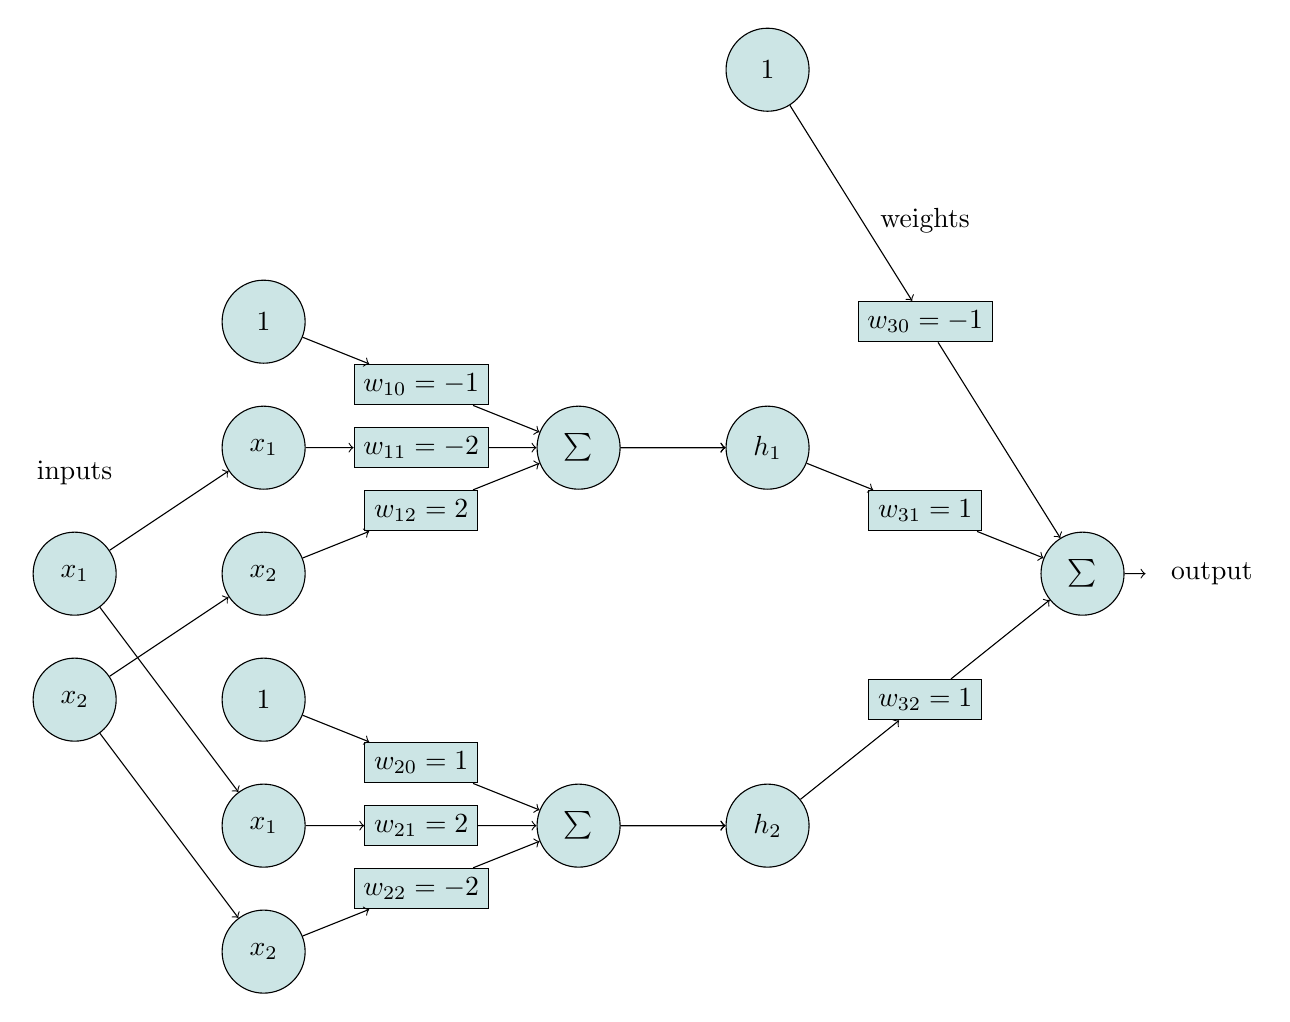
\begin{tikzpicture}[scale=0.8]

    %input x
    \node[input] (x1) at (-3,6){$x_1$};    
    \node[input] (x2) at (-3,4){$x_2$}; 

	% inputs of h1
    \foreach \h [count=\hi ] in {$x_2$,$x_1$,$1$}{
    	\node[input] (f1\hi) at (0,\hi*2cm +4cm) {\h};
    }
    % inputs of h2
    \foreach \h [count=\hi ] in {$x_2$,$x_1$,$1$}{
    	\node[input] (f2\hi) at (0,\hi*2cm -2cm) {\h};
    }
    
    \draw[->] (x1) -- (f12);    
    \draw[->] (x1) -- (f22);  
    \draw[->] (x2) -- (f11);    
    \draw[->] (x2) -- (f21);  
    
	% sum h1
	\node[functions] (sumh1) at (5,8) {$\sum$};
    % sum h2
	\node[functions] (sumh2) at (5,2) {$\sum$};	
	
    % weights of h1
	\foreach \h [count=\hi ] in {$w_{12} =2$,$w_{11} = -2$,$w_{10} = -1$}{%
      	\path (f1\hi) -- node[weights] (w\hi) {\h} (sumh1);
      	\draw[->] (f1\hi) -- (w\hi);
      	\draw[->] (w\hi) -- (sumh1);
    } 
    % weights of h2
	\foreach \h [count=\hi ] in {$w_{22} =-2$,$w_{21} = 2$,$w_{20} = 1$}{%
      	\path (f2\hi) -- node[weights] (w\hi) {\h} (sumh2);
      	\draw[->] (f2\hi) -- (w\hi);
      	\draw[->] (w\hi) -- (sumh2);
    } 
	
	% inputs of g
	\foreach \h [count=\hi ] in {$h_2$,$h_1$,$1$}{%
      \node[input] (h\hi) at (8,\hi*6cm-4 cm) {\h};
    }
    % sum g
	\node[functions] (sumg) at (13,6) {$\sum$};
	% weights of g
	\foreach \h [count=\hi ] in {$w_{32} =1$,$w_{31} = 1$,$w_{30} = -1$}{%
      	\path (h\hi) -- node[weights] (w\hi) {\h} (sumg);
      	\draw[->] (h\hi) -- (w\hi);
      	\draw[->] (w\hi) -- (sumg);
      	\draw[->] (sumh1) -- (h2);
      	\draw[->] (sumh2) -- (h1);
    }        

	\draw[->] (sumg) -- ++(1,0);
	
	% Labels
	\node[above=1cm] at (x1) {inputs};
	\node[above=1cm] at (w3) {weights};
	\node[right=1cm] at (sumg) {output};
\end{tikzpicture}
\caption{Network for question 2b}
\label{fig}
\end{figure}









\subsection{Question 2(c)}

\begin{tabular}{|c|c|c|c|c|c|c|}
\hline
$x_1$ & $x_2$ & $\neg x_1$ & $\neg x_2$ & $x_1 \vee x_2$ & $\neg x_1 \vee \neg x_2$ & $(x_1 \vee x_2)\wedge (\neg x_1 \vee \neg x_2)$\\
\hline
-1 &-1 &1 &1 & -1& 1 & -1\\
-1 &1 &1 &-1 & 1& 1 & 1\\
1 &-1 &-1 &1 & 1& 1 & 1\\
1 &1 &-1 &-1 & 1& -1 & -1\\
\hline
\end{tabular}

Visually this is:

\begin{center}
\begin{tikzpicture}[scale=3.0]
%\draw [help lines] (-3,-3) grid (3,3);
% Euclidean
\draw [<->](0,-1.1)--(0,1.1) node[right]{$x_2$};
\draw [<->](-1.1,0)--(1.1,0) node[right]{$x_1$};
 
\draw[red,thick,dashed] (-1.0,-0.5) -- (0.5,1.0);

%labels
\foreach \x in {-1,1}
     \draw (\x,1pt) -- (\x,-3pt) node[anchor=north] {$\x$};

\foreach \y/\ytext in {-1,1}
     \draw (1pt,\y) -- (-3pt,\y) node[anchor=east] {$\y$};
 
\draw (-1,-1) node[cross,red]{};
\draw (-1,1) node[cross,green]{};
\draw (1,-1) node[cross,green]{};
\draw (1,1) node[cross,red]{}; 

\end{tikzpicture}
\end{center}



\section{Question 3}
\subsection{Question 3(a)}
\subsection{Question 3(b)}
\subsection{Question 3(c)}
\subsection{Question 3(d)}
\subsection{Question 3(e)}

\bibliography{mybib}
\end{document}
